\documentclass[11pt]{article}

\usepackage[margin=1in]{geometry}
\usepackage{booktabs}
\usepackage{graphicx}
\usepackage{amsmath}
\usepackage[hidelinks]{hyperref}
\usepackage{xcolor}
\usepackage{enumitem}
\usepackage{microtype}
\usepackage{siunitx}

\graphicspath{{figures/beta/}{figures/}}

\title{Consensus Consolidation Turns Correct Shared Experience into\\ Silent Strategy Degradation in Multi-Agent LLM Systems}
\author{Phase-Beta results section (draft)}
\date{\today}

\begin{document}
\maketitle

\begin{center}
\fcolorbox{teal!70!black}{teal!5}{\parbox{0.94\linewidth}{%
\textbf{Draft status.} All numbers below come from the preregistered Phase-Beta protocol
(\texttt{prereg\_phase\_beta.md}); gate rules were frozen before data collection and each
verdict is recorded in that document's deviation log. Statistics are same-maze paired
bootstrap (10{,}000 resamples, 95\% CI). Experience text is entirely model-generated; the
sanitizer guarantees no researcher-authored string enters the memory pool.}}
\end{center}

\begin{abstract}
We study whether shared experiential memory in multi-agent LLM systems can turn locally
correct strategies into globally degraded behavior. Using a controlled maze microscope where
every action is legal and shortest-path cost is measurable, we run a preregistered ladder of
experiments with faithful instantiations of ExpeL-style insight operations and
Generative-Agents-style retrieval. We find: (i) at the single-agent level, faithful experience
learning does not measurably change the primary efficiency endpoints (an attribution control);
(ii) at the multi-agent level, injecting experience degrades efficiency and amplifies loops,
with \emph{consensus-consolidated} shared memory producing the most reproducible degradation
across seeds and the only significant loop amplification relative to private memory;
(iii) the harm does not come from read-side usage-weighted retrieval (a null dose-response),
but from write-side consolidation, which compresses the population's active strategy supply by
roughly a factor of two. The failure is silent: agents still succeed, never cross walls, and
never falsely submit, yet increasingly walk in circles.
\end{abstract}

\section{Experimental Ladder and Verdicts}

We evaluate on a generated $15\times15$ trap-maze family (shortest path $\geq 30$) with local
observations, a state-guided controller, and a step cap of 120. Solvers never see the maze graph
or shortest path. Memory conditions differ only in \emph{write protocol} and \emph{sharing};
the reviewer sees agent logs and quality signals, never hidden routes. The primary endpoints,
frozen in advance, are success-only excess steps, loop rate, and the multi-agent ant-mill rate.

\subsection{E1: single-agent attribution control}

Before introducing sharing, we ask whether faithful experience learning changes single-agent
behavior at all. Relative to a no-memory baseline (paired, final round, three seeds), neither the
ExpeL-operations writer nor the append writer moves any primary endpoint: success-only excess
steps CIs contain zero (append $-4.74$, CI $[-14.1, +4.2]$; ops $+5.11$, CI $[-6.4, +16.3]$), as
do loop rates. By the frozen rule this is a \textbf{FAIL}. However, the mandated adherence
analysis shows experience is \emph{not} ignored: the ops writer shifts action selection away from
the controller suggestion after memory activates ($+0.041$ deviation, same sign in $3/3$ seeds),
and the append writer significantly reduces maximum revisits. The single-agent null is therefore
an \emph{attribution control}: any multi-agent degradation cannot be attributed to ``using
memory'' per se, only to the sharing channel.

\subsection{E2: multi-agent memory matrix}

We compare five arms at four agents, $T=6$, five seeds, against a write-only \emph{frozen}
control that accumulates but never injects experience. Table~\ref{tab:e2} and
Figure~\ref{fig:fig2} report paired differences at the final round.

\begin{table}[h]
\centering
\caption{E2 final-round paired differences versus frozen write-only memory (five seeds,
$n_{\text{pairs}}=240$; success-only excess steps drops unpaired failures).
$^\ast$ = 95\% CI excludes zero.}
\label{tab:e2}
\begin{tabular}{lrrrr}
\toprule
Arm & Success & Success excess steps & Loop rate & Max revisits \\
\midrule
MAS no memory      & $-0.004$          & $+1.12$            & $+0.042^\ast$ & $+0.10$ \\
Private memory     & $-0.175^\ast$     & $+7.32^\ast$       & $+0.079^\ast$ & $+1.20^\ast$ \\
Shared append      & $-0.121^\ast$     & $+2.75$            & $+0.025$      & $+0.23$ \\
Shared consolidated& $-0.171^\ast$     & $+11.84^\ast$      & $+0.138^\ast$ & $+1.68^\ast$ \\
\bottomrule
\end{tabular}
\end{table}

Three readings follow. First, multi-agent execution is not itself pathological: MAS-no-memory
matches frozen on efficiency and success, with only a small loop increase
($+0.042$, CI $[0.008, 0.075]$). Second, \textbf{consensus-consolidated shared memory meets every
preregistered degradation criterion}: success-only excess steps $+11.84$ (CI $[7.66, 16.02]$),
same-sign in $5/5$ seeds and \emph{larger} in the later seeds; loop rate $+0.138$
(CI $[0.092, 0.188]$); success $-0.171$. Third, the broad risk is active injection rather than
sharing alone---private memory also degrades---so we test the sharing-specific claim directly.

\paragraph{Shared versus private boundary.} Figure~\ref{fig:fig2b} contrasts the shared arms
against a \emph{private} baseline. The efficiency separation is not significant
(consolidated vs private success-only excess steps $+0.87$, CI $[-4.29, +6.15]$), but loop
amplification is: consolidated loops significantly more than private ($+0.058$,
CI $[0.008, 0.113]$), while append loops \emph{less}. The honest claim is therefore that
consensus consolidation specifically amplifies looping relative to private memory; we do not
claim a broad shared-over-private efficiency gap.

\subsection{E3: read-side dose-response is null}

If the harm were read-side---agents increasingly retrieving a few high-vote memories---then
raising the importance weight $\lambda$ in Generative-Agents-style scoring should deepen
degradation. It does not. Sweeping $\lambda\in\{0,0.5,1\}$ on the append arm (three seeds,
$T=6$), the paired difference of $\lambda{=}1$ versus $\lambda{=}0$ on success-only excess steps
is $+1.69$ (CI $[-4.26, +7.61]$), loop rate $+0.049$ (CI $[0.000, 0.104]$), and final-round
retrieval entropy is non-monotone in $\lambda$ ($0.833/0.826/0.845$). The read-side
usage-weighted-feedback hypothesis is \textbf{refuted}; we report it as a clean null.

\subsection{Mechanism: write-side strategy-supply compression}

An offline audit of the same E2 runs locates the concentration on the \emph{write} side
(Figure~\ref{fig:fig3}). Under identical settings, the consolidated pool converges to
$14.2$ items with only $11.0$ distinct experiences ever injected across all rounds, whereas the
append pool grows to the cap ($80$) and injects $25.4$ distinct experiences, and private injects
$37.6$. Consensus consolidation compresses the population's active strategy supply by roughly
$2.3\times$ relative to append. The top-1 retrieval share rises in step, but this is a
consequence of the smaller pool rather than an independent channel; the load-bearing evidence is
the direct pool-size and distinct-injection counts.

\section{The Failure Is Silent}

Figure~\ref{fig:fig1} shows the mechanism schematic and a case study mined from the runs: the
same held-out maze and agent at the final round, whose shortest path is 38 steps. As the write
protocol consolidates, the route degrades monotonically---frozen 39 steps (one revisit),
private 47 (four), shared-append 55 (nine), shared-consolidated 73 with cost 1.92, eleven revisits
to the same cell, and a detected loop---yet every route is legal and every arm still reaches the
goal. This is the ant-mill signature: not a false belief, but a locally plausible correction
signal, reinforced through consensus writing, that composes into a globally wasteful cycle.

\section{Summary of Claims}

\begin{itemize}[leftmargin=1.4em]
\item Single-agent faithful experience learning does not move the primary endpoints (attribution
control; E1).
\item Multi-agent experience injection degrades efficiency and amplifies loops; consensus
consolidation is the most reproducible degrading arm across seeds (E2).
\item Relative to private memory, the shared-specific effect is loop amplification, not a broad
efficiency gap (E2 boundary).
\item The harm is not read-side usage-weighted retrieval (null dose-response; E3) but write-side
consolidation that compresses the active strategy supply (mechanism audit).
\end{itemize}

% ---------------------------------------------------------------- figures
\begin{figure}[p]
\centering
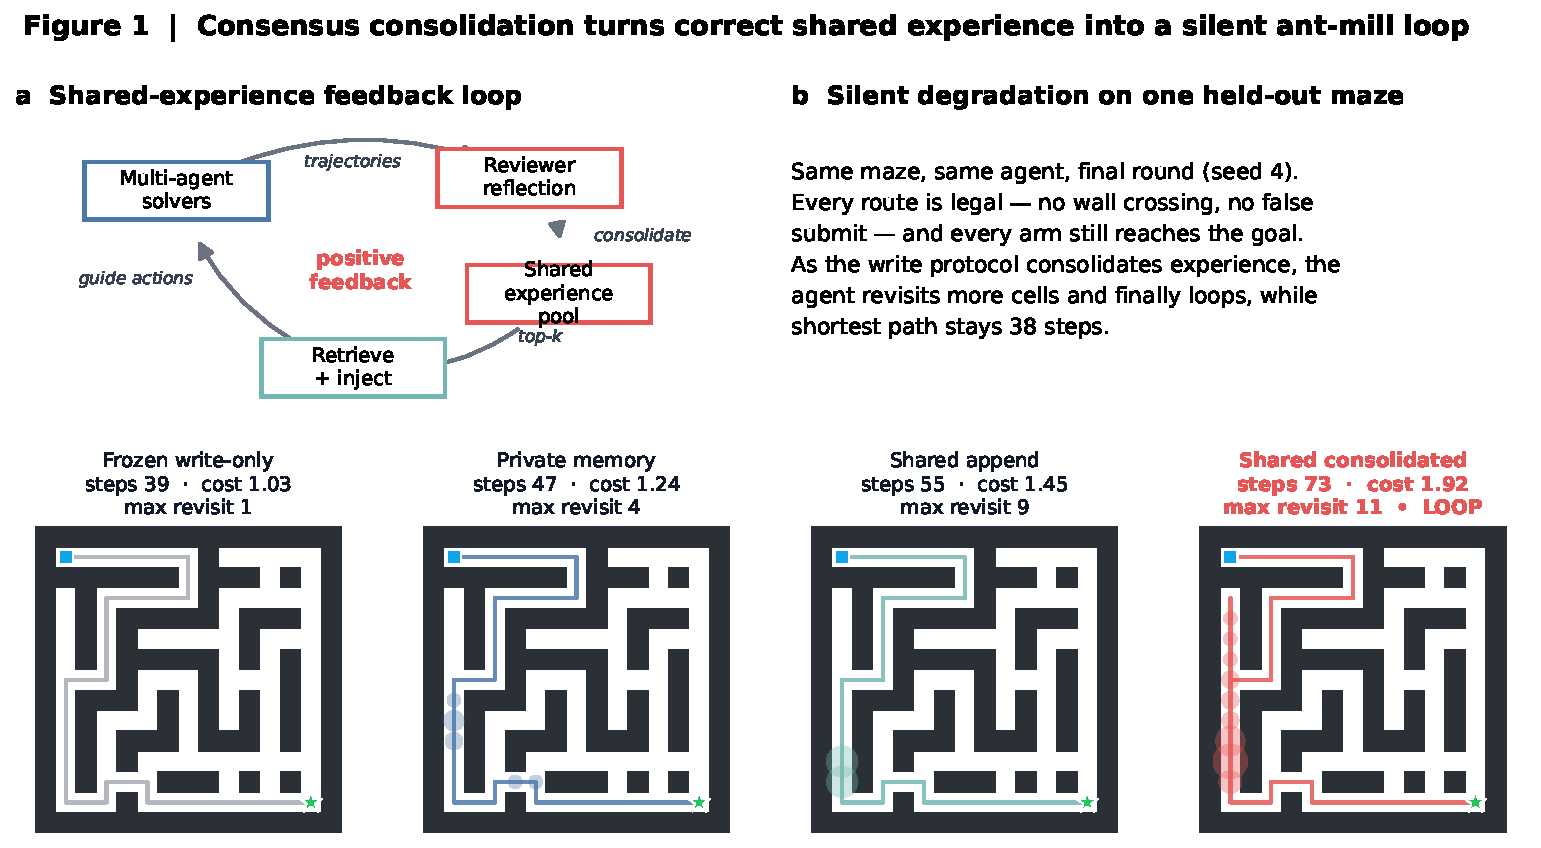
\includegraphics[width=\linewidth]{figure1_mechanism.pdf}
\caption{\textbf{Mechanism microscope and a silent degradation case.}
(a) The shared-experience feedback loop: solver trajectories are reflected into a shared pool,
consolidated by LLM-issued operations, retrieved top-$k$, and injected back as guidance---a
positive-feedback cycle. (b) Same held-out maze and agent, final round; shortest path 38.
Revisit heat (shaded blobs) grows as the write protocol consolidates, culminating in a silent
loop under shared-consolidated memory, while every route stays legal and successful.}
\label{fig:fig1}
\end{figure}

\begin{figure}[p]
\centering
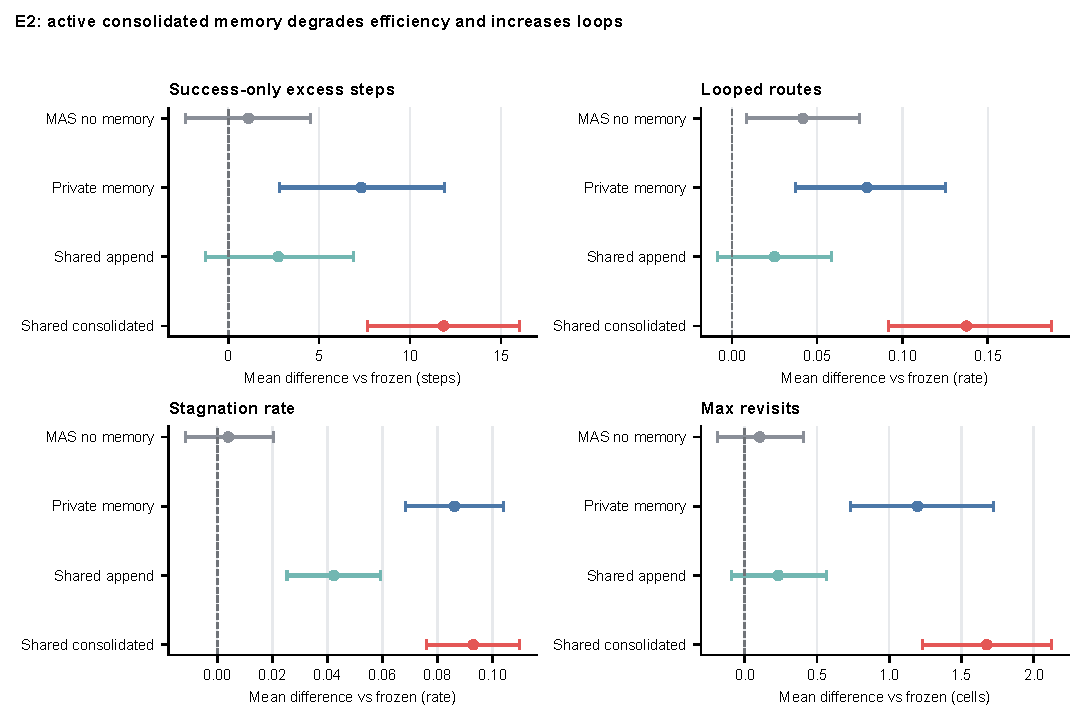
\includegraphics[width=\linewidth]{figure2_e2_main.pdf}
\caption{\textbf{E2 main result: paired differences versus frozen write-only memory}
(five seeds, final round). Points are mean differences; bars are 95\% bootstrap CIs; the dashed
line is zero. Shared-consolidated (red) degrades on all four endpoints with the largest effects;
MAS-no-memory (grey) is on the zero line except for a small loop increase.}
\label{fig:fig2}
\end{figure}

\begin{figure}[p]
\centering
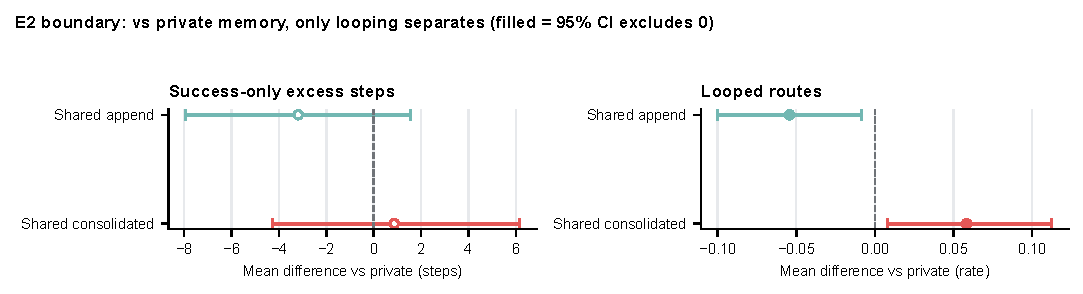
\includegraphics[width=\linewidth]{figure2b_shared_vs_private.pdf}
\caption{\textbf{E2 boundary: shared arms versus a private baseline.}
Filled markers mark CIs that exclude zero. Only looping separates shared-consolidated from
private ($+0.058$, CI $[0.008, 0.113]$); the efficiency contrast does not, and shared-append
actually loops less than private.}
\label{fig:fig2b}
\end{figure}

\begin{figure}[p]
\centering
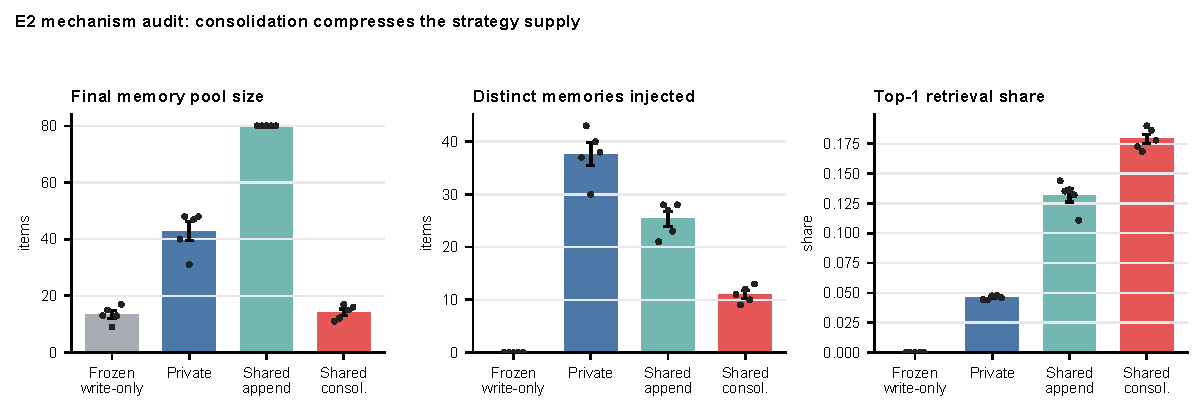
\includegraphics[width=\linewidth]{figure3_write_side_compression.pdf}
\caption{\textbf{Mechanism audit: consolidation compresses the strategy supply.}
Final pool size, distinct experiences ever injected, and top-1 retrieval share across five seeds
(dots). Consensus consolidation keeps a small pool and injects the fewest distinct strategies,
concentrating retrieval; the direct counts (left, centre) carry the causal claim.}
\label{fig:fig3}
\end{figure}

\end{document}
